\documentclass[aspectratio=169]{beamer}

% Base theme
\usetheme{CambridgeUS}
\usecolortheme{default}

% Page numbers, no nav symbols
\setbeamertemplate{footline}{%
  \hfill\small\insertframenumber\,/\,\inserttotalframenumber\hspace*{2mm}\vspace*{1mm}%
}
\setbeamertemplate{navigation symbols}{}

% Packages
\usepackage{xcolor}
\usepackage{booktabs}
\usepackage{graphicx}
\usepackage{hyperref}
\usepackage{amsmath, amssymb}

% --- UGA color scheme ---
\definecolor{UGARed}{HTML}{BA0C2F}
\definecolor{UGABlack}{HTML}{000000}

\setbeamercolor{structure}{fg=UGARed}
\setbeamercolor{frametitle}{fg=UGABlack}
\setbeamercolor{title}{fg=UGABlack}
\setbeamercolor{normal text}{fg=UGABlack}
\setbeamercolor{itemize item}{fg=UGARed}
\setbeamercolor{itemize subitem}{fg=UGARed}
\setbeamercolor{section in toc}{fg=UGABlack}
\setbeamercolor{section in toc shaded}{fg=UGABlack!30}
\setbeamercolor{subsection in toc}{fg=UGABlack}
\setbeamercolor{subsection in toc shaded}{fg=UGABlack!30}

% Slightly tighter lists
\setbeamertemplate{itemize items}[circle]
\setlength{\itemsep}{4pt}

% Title info
\title{(Breaking) Intergenerational Transmission of Mental Health}
\subtitle{}
\author{B\"{u}tikofer, Ginja, Karbownik, and Landaud (JHR 2023)}
\institute{University of Georgia}
\date{\today}

% Section roadmap slides (excluded from frame count)
\AtBeginSection[]{
  \begin{frame}[plain, noframenumbering]{Outline}
    \tableofcontents[currentsection, sectionstyle=show/shaded, subsectionstyle=show/show/shaded]
  \end{frame}
}

\begin{document}

% Title slide (excluded from frame count)
\begin{frame}[plain, noframenumbering]
  \titlepage
\end{frame}

% -------------------------------------------------------
\section{Motivation}
% -------------------------------------------------------

\begin{frame}{The Global Mental Health Burden}
  \begin{itemize}
    \item Mental health disorders affect \textbf{more than one billion people worldwide}
    \item Among leading causes of disability and rising share of global disease burden
    \item Economic costs are large and growing:
    \begin{itemize}
      \item US: \$201 billion in 2013; projected \$225 billion by 2019
      \item Norway: NOK32 billion (\$3.7B USD) in 2013; NOK65 billion by 2023
    \end{itemize}
    \item COVID-19 has further exacerbated demand for mental health care
    \item True economic costs exceed medical spending: productivity loss, forgone taxes, externalities on others
  \end{itemize}
\end{frame}

\begin{frame}{An Understudied Externality: Intergenerational Transmission}
  \begin{itemize}
    \item One key externality is the intergenerational association between parent and child mental health
    \item If mental health conditions transmit across generations, costs imposed on future generations are substantial and unaccounted for
    \item Three research questions:
    \begin{itemize}
      \item What is the \textbf{association} between parent and child mental health?
      \item How different is it from physical health? How important is the \textbf{extended family}?
      \item Can a \textbf{targeted low-touch policy} break the intergenerational link?
    \end{itemize}
    \item Answers require: population-level data, objective health measures, family linkages across generations
  \end{itemize}
\end{frame}

\begin{frame}{Preview of Main Findings}
  \begin{itemize}
    \item \textbf{Persistence is large:} having a parent with a mental health diagnosis raises child's probability of mental health diagnosis by 9.3 percentage points (40\% of control mean)
    \item \textbf{Dynasty matters:} focusing only on parents understates persistence by 42\% --- extended family adds substantial explanatory power
    \item \textbf{Mental $\approx$ physical:} intergenerational associations in mental and physical health are broadly similar in magnitude; genetics likely not the full story
    \item \textbf{Policy can help:} a 2007 Norwegian pilot program reduced the parent-child mental health association by 39\%
    \begin{itemize}
      \item Larger effects for children of college-educated parents; raises equity concerns
    \end{itemize}
  \end{itemize}
\end{frame}

% -------------------------------------------------------
\section{Related Literature and Contribution}
% -------------------------------------------------------

\begin{frame}{Prior Literature on Intergenerational Health}
  \begin{itemize}
    \item \textbf{General health persistence:} Andersen (2021), Bj\"{o}rkegren et al.\ (2022), Halliday et al.\ (2021) --- registry-based estimates tend to be smaller than survey-based
    \item \textbf{Specific conditions:} birth weight (Currie \& Moretti 2003), cardiovascular (Lloyd-Jones et al.\ 2004), BMI (Classen 2010)
    \item \textbf{Mental health specifically is scarcer:}
    \begin{itemize}
      \item Survey-based: Johnston, Schurer, \& Shields (2013); Bencsik, Halliday, \& Mazumder (2021); Vera-Toscano \& Brown (2021)
      \item Specific disorders: Akbulut-Yuksel \& Kugler (2016) for depression; Eley et al.\ (2015) for anxiety
      \item Almost all rely on \textbf{self-reported survey data}: recall bias, small samples, ordered intervals
    \end{itemize}
    \item Survey estimates of parent-child mental health ICs: 0.13 (Johnston et al.) to 0.22 (Bencsik et al.)
    \item Only Andersen (2021) provides population-level estimates using administrative GP/hospitalization data for Denmark
  \end{itemize}
\end{frame}

\begin{frame}{This Paper's Contribution}
  \begin{itemize}
    \item Connects three literatures:
    \begin{enumerate}
      \item \textbf{Intergenerational health persistence}: adds administrative mental health, dynasty component, causal policy variation
      \item \textbf{Dynastic human capital} (Adermon, Lindahl \& Palme 2021): replicates for Norway, extends beyond education to health outcomes
      \item \textbf{Health interventions in childhood}: Hj\o{}rt, S\o{}lvsten, \& W\"{u}st (2017); B\"{u}tikofer \& Salvanes (2020); Baranov et al.\ (2020) --- light-touch policies can reduce persistent disadvantage
    \end{enumerate}
    \item Broader implication: standard program evaluations that stop at the directly treated generation \textbf{may understate returns} to mental health investments
  \end{itemize}
\end{frame}

% -------------------------------------------------------
\section{Setting and Data}
% -------------------------------------------------------

\begin{frame}{Why Norway?}
  \begin{itemize}
    \item Healthcare is \textbf{highly subsidized and universally accessible} --- limits selection into treatment based on income
    \item Unique \textbf{personal and family identifiers} across all administrative registers: link individuals across four generations
    \item General practitioners (GPs) and primary care ER doctors are \textbf{obligated to report all consultations}
    \begin{itemize}
      \item Near-universal coverage for children 13--18: 91\% visited primary healthcare before seeing a specialist
    \end{itemize}
    \item Reduces concerns about underreporting relative to survey data:
    \begin{itemize}
      \item Bharadwaj, Pai, and Suzie-delyte (2017): large underreporting of MH in surveys vs.\ administrative records
    \end{itemize}
    \item Private insurance/clinics have negligible market share ($\approx$ 10,000 adults with private coverage in 2003)
  \end{itemize}
\end{frame}

\begin{frame}{Data Sources}
  \begin{itemize}
    \item \textbf{Family registers (1992--2015):} link parents, children, and extended family via birth certificates; construct extended family horizontally (siblings, cousins, spouses)
    \item \textbf{KUHR --- Control and Payment of Health Refunds (2006--2020):} children's health
    \begin{itemize}
      \item GP and primary care ER visits; ICPC-2 coded
      \item Available from 2006 onward
    \end{itemize}
    \item \textbf{Social Security sickness leave registry (1992+):} parental health
    \begin{itemize}
      \item All absences $>3$ days certified by a physician; ICPC-2 coded
    \end{itemize}
    \item \textbf{Demographic, education, and income registers:} controls and heterogeneity analyses
  \end{itemize}
\end{frame}

\begin{frame}{Measuring Mental Health}
  \textbf{Children's Mental Health:}
  \begin{itemize}
    \item \textbf{Source:} KUHR registry --- GP and ER visits between ages 13 and 18
    \item \textbf{Mental health indicator:} any GP or ER visit with an ICPC-2 code starting with the letter ``P''
  \end{itemize}
  \textbf{Parents' Mental Health:}
  \begin{itemize}
    \item \textbf{Source:} Sickness leave registry --- any physician-certified sickness leave for mental health reasons (ICPC-2 code ``P'') at ages 25--30
    \item \textbf{Why this window:} ensures parental health is measured \textit{before} the child's outcome window (ages 13--18)
    \item 7\% of mothers and 4\% of fathers take at least one MH sickness leave at ages 25--30
    \item Most common MH condition: depression (both genders)
  \end{itemize}
\end{frame}

\begin{frame}{Limitations of the Sickness Leave Measure}
  \begin{itemize}
    \item \textbf{Eligibility constraint:} only individuals in the labor market qualify --- 6\% of 25--30 year olds ineligible
    \begin{itemize}
      \item Ineligibility more common among foreign-born, lower-income individuals
      \item Our estimates likely represent an \textbf{upper bound} for severe conditions (sickest may not work); a \textbf{lower bound} for mild conditions (mild cases may not take leave)
    \end{itemize}
    \item \textbf{Severity truncation:} not all mental health episodes lead to leave --- depression manageable by medication may not appear
    \item \textbf{Coverage overlap:} for 2006--2008, compare sickness leave to KUHR data: 23\% of individuals with a MH event in KUHR took sickness leave
    \item \textbf{External validity:} parents with MH diagnoses are somewhat more likely to be parents than those without, suggesting our sample is not severely selected
    \item Robustness: control for sickness leave eligibility determinants (education, income, immigration status) --- results unchanged
  \end{itemize}
\end{frame}

\begin{frame}{Constructing the Extended Family (Dynasty)}
  \begin{itemize}
    \item Following Adermon, Lindahl, and Palme (2021): define the dynasty to include \textbf{five branches} of the extended family beyond parents:
    \begin{enumerate}
      \item \textbf{Parents' siblings} (sp) --- 25\% genes shared
      \item \textbf{Spouses of parents' siblings} (ssp) --- plausibly unrelated genetically
      \item \textbf{Siblings of spouses of parents' siblings} (sssp) --- plausibly unrelated
      \item \textbf{Parents' cousins} (cp) --- 12.5\% genes shared
      \item \textbf{Spouses of parents' cousins} (scp) --- plausibly unrelated
    \end{enumerate}
    \item Associations for ``plausibly unrelated'' members (ssp, sssp, scp) constitute 18--15\% of total intergenerational persistence $\Rightarrow$ genetics alone cannot explain the full picture
    \item Control for \textbf{number of members} in each branch of extended family to avoid mechanical effects
  \end{itemize}
\end{frame}

\begin{frame}{Sample Selection and Descriptive Statistics}
  \begin{itemize}
    \item Start: all children born in Norway 1988--2007, resident ages 13--18 in 2006--2020 ($N = 732{,}437$)
    \item Restrict to:
    \begin{itemize}
      \item Parents with labor income at ages 25--30 (sickness leave eligibility): drop 4,907
      \item Children with known grandparents and great-grandparents: $N = 370{,}498$ preferred sample
    \end{itemize}
    \item \textbf{Children:} 24\% have any MH diagnosis; 6.96\% have depression; 51\% male
    \item \textbf{Mothers:} 54\% take at least one sickness leave ages 25--30; 7\% for MH reasons; most common reason: musculoskeletal (23\%)
    \item \textbf{Fathers:} 28\% take at least one sickness leave; 4\% for MH reasons
    \item Parent-child MH correlations below 0.04 in the raw data (Pearson) --- associations are real but moderate
  \end{itemize}
\end{frame}

\begin{frame}{Sample Statistics}
  \scriptsize
  \begin{table}
  \centering
  \begin{tabular}{lcccc}
  \toprule
  & \multicolumn{2}{c}{All Children} & \multicolumn{2}{c}{Analysis Sample} \\
  \cmidrule(lr){2-3}\cmidrule(lr){4-5}
  & Mean & SD & Mean & SD \\
  \midrule
  \multicolumn{5}{l}{\textit{Panel A: Children}} \\
  Any MH diagnosis          & 23.09 & 42.14 & 24.00 & 42.71 \\
  Depression                & 6.72  & 25.03 & 6.96  & 25.45 \\
  Any specialist care (MH)  & 4.03  & 19.67 & 4.11  & 19.85 \\
  Male                      & 0.51  & 0.50  & 0.51  & 0.50  \\
  GPA                       & 4.09  & 0.82  & 4.05  & 0.83  \\
  $\geq 1$ parent college   & 0.36  & 0.48  & 0.33  & 0.47  \\
  \midrule
  \multicolumn{5}{l}{\textit{Panel B: Mother}} \\
  Any sick leave (25--30)   & 0.50  & 0.50  & 0.54  & 0.50  \\
  Any MH sick leave (25--30)& 0.06  & 0.24  & 0.07  & 0.26  \\
  Any depression SL (25--30)& 0.04  & 0.20  & 0.05  & 0.21  \\
  \midrule
  \multicolumn{5}{l}{\textit{Panel C: Father}} \\
  Any sick leave (25--30)   & 0.26  & 0.44  & 0.28  & 0.45  \\
  Any MH sick leave (25--30)& 0.03  & 0.18  & 0.04  & 0.19  \\
  Any depression SL (25--30)& 0.02  & 0.14  & 0.02  & 0.14  \\
  \bottomrule
  \multicolumn{5}{p{0.85\linewidth}}{\scriptsize Children's health measured ages 13--18; parental health at ages 25--30. $N=370{,}498$ (analysis sample).}
  \end{tabular}
  \end{table}
\end{frame}


% -------------------------------------------------------
\section{Empirical Framework}
% -------------------------------------------------------

\begin{frame}{Econometric Model: Intergenerational Persistence}
  \small
  Regress child mental health on parental and extended family mental health:
  \[
    Y_{it} = \alpha + \beta_p Y^p_{t-1} + \sum_{k \in \{sp,\, cp,\, ssp,\, sssp,\, scp\}} \beta_k Y^k_{t-1} + \gamma \mathbf{X}_{it} + \varepsilon_{it}
  \]
  \begin{itemize}
    \item $Y_{it}$: indicator (extensive) or count (intensive) of child's MH events, ages 13--18, $\times 100$
    \item $Y^p_{t-1}$: parental MH sickness leave, ages 25--30 (measured before child outcome)
    \item $Y^k_{t-1}$: MH sickness leave of extended family branch $k$
    \item $\mathbf{X}_{it}$: year of birth FE, year first observed in KUHR, gender, number of individuals per dynasty branch; \emph{select specs} add SES controls
    \item Parameters of interest: $\beta_p$ (parent-child) and $\beta_k$ (extended family)
    \item Standard errors: Eicker-Huber-White, clustered at the family level
  \end{itemize}
\end{frame}

\begin{frame}{Identification: What We Can and Cannot Claim}
  \begin{itemize}
    \item \textbf{What the design delivers:} associations / correlations between parent and child MH, not causal effects of parental MH on child MH
    \item These associations are policy-relevant regardless of mechanism:
    \begin{itemize}
      \item Mental health diagnoses trigger initial treatment and follow-up costs
      \item They motivate the targeted intervention in Section V
    \end{itemize}
    \item \textbf{Timing:} parental health measured at ages 25--30, strictly before child's outcome window (ages 13--18) $\Rightarrow$ rules out co-diagnosis
    \item \textbf{Not causal but informative:} associations are robust to controlling for SES, school FE, GP FE, prenatal health, and birth characteristics
    \item Cannot separate genetic from social/environmental channels --- dynasty analysis provides suggestive evidence that social factors matter
  \end{itemize}
\end{frame}

\begin{frame}{A Note on Measurement of Parental Health}
  \begin{itemize}
    \item \textbf{Upper vs.\ lower bound concern:}
    \begin{itemize}
      \item If milder conditions have lower persistence $\Rightarrow$ sicker individuals more likely captured $\Rightarrow$ estimates are an \textbf{upper bound}
      \item If sickest individuals exit the labor market $\Rightarrow$ most severe cases missed $\Rightarrow$ estimates are a \textbf{lower bound}
    \end{itemize}
    \item Authors conclude: upper bound concern is more plausible given the data
    \item \textbf{Validate} with 2006--2008 overlap of KUHR and sickness leave: 23\% of individuals with a MH symptom in KUHR took sickness leave
    \item \textbf{Administrative vs.\ survey:} Bharadwaj et al.\ (2017) show large underreporting of MH in surveys --- administrative records likely more accurate
  \end{itemize}
\end{frame}

\begin{frame}{Dynastic Correlations in Mental Health (Extensive Margin)}
  \scriptsize
  \begin{tabular}{lcccc}
  \toprule
  & (1) & (2) & (3) & (4) \\
  & Parents only & $+$ Siblings & Full dynasty & $+$ Physical health \\
  \midrule
  Parents' MH
    & 9.805$^{***}$ & 9.664$^{***}$ & 9.569$^{***}$ & 9.257$^{***}$ \\
    & (0.254) & (0.254) & (0.254) & (0.255) \\
  Parents' siblings MH
    & & 2.990$^{***}$ & 2.848$^{***}$ & 2.557$^{***}$ \\
    & & (0.208) & (0.208) & (0.210) \\
  Spouses of parents' siblings MH
    & & & 1.417$^{***}$ & 1.181$^{***}$ \\
    & & & (0.256) & (0.258) \\
  Parents' cousins MH
    & & & 1.654$^{***}$ & 1.475$^{***}$ \\
    & & & (0.163) & (0.164) \\
  Spouses of parents' cousins MH
    & & & 0.676$^{***}$ & 0.556$^{***}$ \\
    & & & (0.195) & (0.195) \\
  Siblings of spouses of parents' siblings MH
    & & & 1.025$^{***}$ & 0.883$^{***}$ \\
    & & & (0.206) & (0.208) \\
  \midrule
  Control for physical health & No & No & No & Yes \\
  Control mean & \multicolumn{4}{c}{22.9} \\
  Sum of coefficients & 9.8 & 12.7 & 17.2 & 15.9 \\
  $R^2$ & 0.052 & 0.052 & 0.053 & 0.053 \\
  $N$ & \multicolumn{4}{c}{370,498} \\
  \bottomrule
  \end{tabular}
\end{frame}

\begin{frame}{Dynastic Correlations in Mental Health: Intensive Margin}
\scriptsize
\begin{tabular}{lcccc}
\toprule
 & (1) & (2) & (3) & (4) \\
 & Parents only & $+$ Siblings & Full dynasty & $+$ Physical health \\
\midrule
Parents' MH
  & 0.050$^{***}$ & 0.050$^{***}$ & 0.049$^{***}$ & 0.048$^{***}$ \\
  & (0.003) & (0.003) & (0.003) & (0.003) \\
Parents' siblings MH
  & & 0.017$^{***}$ & 0.017$^{***}$ & 0.016$^{***}$ \\
  & & (0.002) & (0.002) & (0.002) \\
Sp.\ of par.\ siblings MH
  & & & 0.007$^{***}$ & 0.006$^{***}$ \\
  & & & (0.002) & (0.002) \\
Parents' cousins MH
  & & & 0.007$^{***}$ & 0.006$^{***}$ \\
  & & & (0.002) & (0.002) \\
Sp.\ of par.\ cousins MH
  & & & 0.002 & 0.002 \\
  & & & (0.002) & (0.002) \\
Sib.\ of sp.\ of par.\ siblings MH
  & & & 0.004$^{**}$ & 0.003$^{*}$ \\
  & & & (0.002) & (0.002) \\
\midrule
Control for physical health & No & No & No & Yes \\
Sum of coefficients & 0.050 & 0.067 & 0.085 & 0.080 \\
$R^2$ & 0.032 & 0.032 & 0.032 & 0.034 \\
$N$ & \multicolumn{4}{c}{370,498} \\
\bottomrule
\end{tabular}
\end{frame}
% -------------------------------------------------------
\section{Intergenerational Persistence in Health}
% -------------------------------------------------------

\begin{frame}{Main Results: Extensive Margin (Mental Health)}
  \begin{itemize}
    \item \textbf{Parent-child association (Column 1):} 9.8 percentage points
    \begin{itemize}
      \item Control group mean = 23\% $\Rightarrow$ this is a \textbf{40\% increase} in the probability of a MH event
    \end{itemize}
    \item Adding extended family branches: parent coefficient barely changes
    \begin{itemize}
      \item Parent-child association is largely \textbf{orthogonal} to extended family associations
    \end{itemize}
    \item \textbf{Full dynastic model (Column 3):} parent coefficient = 9.6 pp; sum of all extended family = 7.6 pp $\Rightarrow$ dynasty adds 79\% more
    \item \textbf{Controlling for physical health (Column 4):} parent coefficient = 9.3 pp --- MH associations not driven by cross-condition correlations
    \item All extended family branches are statistically significant; magnitude decreasing in familial distance
  \end{itemize}
\end{frame}

\begin{frame}{Main Results: Intensive Margin}
  \begin{itemize}
    \item Substitute indicator variables with \textbf{standardized counts} of MH health events (children) and MH sickness leave days (parents and extended family)
    \item \textbf{Parent-child association:} 0.05 standard deviations (extensive: $\approx 0.05$ too) --- broadly comparable
    \item \textbf{Extended family:} sum of coefficients = 0.037, or 75.5\% of the parent-child association
    \begin{itemize}
      \item Very similar ratio to the extensive margin
    \end{itemize}
    \item Spouses of parents' cousins (scp) becomes statistically insignificant in the intensive margin saturated model
    \item Physical health intensive margin: sum of extended family = 76.3\% of parent-child association --- nearly identical to mental health
    \item Intergenerational health elasticities (intensive margin): \textbf{0.05 for MH}, 0.06 for physical health
    \begin{itemize}
      \item Grows to 0.09--0.10 when dynasty is included
      \item Substantially smaller than socioeconomic outcomes (income 0.34, wealth 0.35, education 0.25)
    \end{itemize}
  \end{itemize}
\end{frame}

\begin{frame}{Dynastic Effects: Why the Extended Family Matters}
  \begin{itemize}
    \item Ignoring dynasty \textbf{underestimates} total intergenerational persistence by 42\%
    \item Extended family associations decrease with genetic distance:
    \begin{itemize}
      \item Parents' siblings (sp): 14.8\% of parent-child association
      \item Spouses of parents' siblings (ssp): 7.1\% --- plausibly unrelated genetically
      \item Spouses of parents' siblings and their siblings: smallest, but still significant
    \end{itemize}
    \item ``Plausibly unrelated'' members (ssp, sssp, scp) account for 18\% of total extensive MH persistence
    \begin{itemize}
      \item Suggests social mechanisms (modeling behavior, resources, awareness) matter --- not purely genetic
    \end{itemize}
    \item Contrast with \textbf{educational persistence:} dynastic educational associations constitute only 6\% of the corresponding parent-child association
    \item Mental health is more ``visible'' within extended families than education --- may enable social transmission
  \end{itemize}
\end{frame}

\begin{frame}{Physical vs.\ Mental Health Persistence}
  \begin{itemize}
    \item \textbf{Prior literature} often assumes mental $\neq$ physical health in intergenerational persistence (different mechanisms, heritability)
    \item \textbf{This paper's finding:} MH and physical health (OH) associations are largely similar
    \begin{itemize}
      \item Extensive margin: parent-child MH IC = 0.050, OH IC = 0.062 --- modestly larger for physical health
      \item Intensive margin: nearly identical magnitudes
    \end{itemize}
    \item MH associations are unaffected by controlling for physical health of generation $t-1$ (and vice versa)
    \item Extended family patterns mirror each other: parent-child association independent of dynasty for both MH and OH
    \item Implication: the mechanisms driving intergenerational health persistence --- genetic, social, environmental --- are not fundamentally different across MH and OH
  \end{itemize}
\end{frame}

\begin{frame}{Comparing Health and Educational Persistence}
  \begin{itemize}
    \item Replicate Adermon, Lindahl, and Palme (2021) for Norway using Grade 10 GPA as outcome
    \item \textbf{Parent-child education elasticity:} 0.45 --- nine times larger than MH (0.05)
    \item \textbf{Dynasty sum for education:} 0.549 in Norway (vs.\ 0.518 in Sweden)
    \item Dynastic education associations \textbf{do not change} even when controlling for dynastic health associations
    \begin{itemize}
      \item Education and health channels are separate --- health does not mediate educational transmission
    \end{itemize}
    \item ``Genetically unrelated'' dynastic members matter more for health (18\%) than for education (6\%)
    \begin{itemize}
      \item Mental and physical health issues may be more ``visible'' within extended families than education, enabling social transmission
    \end{itemize}
  \end{itemize}
\end{frame}

\begin{frame}{Magnitudes Relative to Prior Literature}
  \begin{itemize}
    \item Administrative data estimates tend to be \textbf{two to four times smaller} than survey estimates
    \begin{itemize}
      \item U.K.\ survey ICs: 0.13--0.22 (Johnston et al.; Bencsik et al.)
      \item This paper (Norway, admin): parent-child IC $\approx 0.05$ (intensive margin)
    \end{itemize}
    \item Consistent with other registry-based work:
    \begin{itemize}
      \item Bj\"{o}rkegren et al.\ (2022): 0.11--0.14 using hospitalizations in Sweden
      \item Andersen (2021): 0.09--0.14 for general health in Denmark
    \end{itemize}
    \item Likely explanations for gap vs.\ surveys:
    \begin{itemize}
      \item Upward bias from recall, subjective perception, Likert scale in survey data
      \item Norway's universal healthcare reduces selection into treatment
    \end{itemize}
    \item Norway is not an outlier: OECD data suggest comparable MH burden to other developed countries
  \end{itemize}
\end{frame}

% -------------------------------------------------------
\section{Targeted Policy and Breaking the Cycle}
% -------------------------------------------------------

\begin{frame}{The 2007 Pilot Program: Modellkommunefors\o{}ket}
  \begin{itemize}
    \item In 2007, the Norwegian Directorate for Children, Youth, and Family Affairs launched a \textbf{pilot in 26 municipalities}
    \item Goal: find best practices for supporting young children (ages 0--6) of parents with mental health conditions
    \item Municipalities received NOK100,000--290,000 annually from central government
    \item The program was \textbf{light-touch and varied} across municipalities:
    \begin{itemize}
      \item Screening tools for psychological distress among targeted children
      \item Establishing specialist teams and interagency cooperation
      \item Childcare center psychologists; home visits; parenting programs (PMTO)
      \item Family coordination and case managers
    \end{itemize}
    \item By 2010, all pilot municipalities had a registration system and screening tools
    \item Success led to a \textbf{2010 national law} mandating similar practices across all Norwegian municipalities
  \end{itemize}
\end{frame}

\begin{frame}{Empirical Strategy: Triple Differences}
  \small
  Since 26 out of 428 municipalities were not chosen randomly, use a \textbf{triple differences} design:
  \[
  \begin{align}
    Y_{icm} \; &= \alpha + \beta(E_{ic} \times D_{im} \times MPH_i) + \delta_1 MPH_i + \delta_2(E_{ic} \times MPH_i) + \delta_3(D_{im} \times MPH_i) \\
              & + \delta_4(E_{ic} \times D_{im}) + \mathbf{X}_i' \boldsymbol{\mu} + \rho_c + \pi_m + \varepsilon_{icm}
  \end{align}
  \]
  \begin{itemize}
    \item $Y_{icm}$: any MH GP/ER visit ages 13--18 for child $i$, cohort $c$, municipality $m$ ($\times 100$)
    \item $MPH_i$: indicator for parental MH diagnosis (2000--2010)
    \item $D_{im}$: indicator for treated municipality
    \item $E_{ic}$: indicator for child aged $\leq 6$ in 2007 (eligible cohort)
    \item \textbf{$\beta$}: ITT estimate of how the program affects the parent-child MH association
    \item Controls: year of birth FE, municipality FE, child gender, parent ages, birth weight, birth rank, parental education
    \item Municipalities matched via Mahalanobis distance on pre-intervention characteristics
  \end{itemize}
\end{frame}

\begin{frame}{Credibility: Parallel Trends and Placebo Tests}
  \begin{figure}
    \centering
    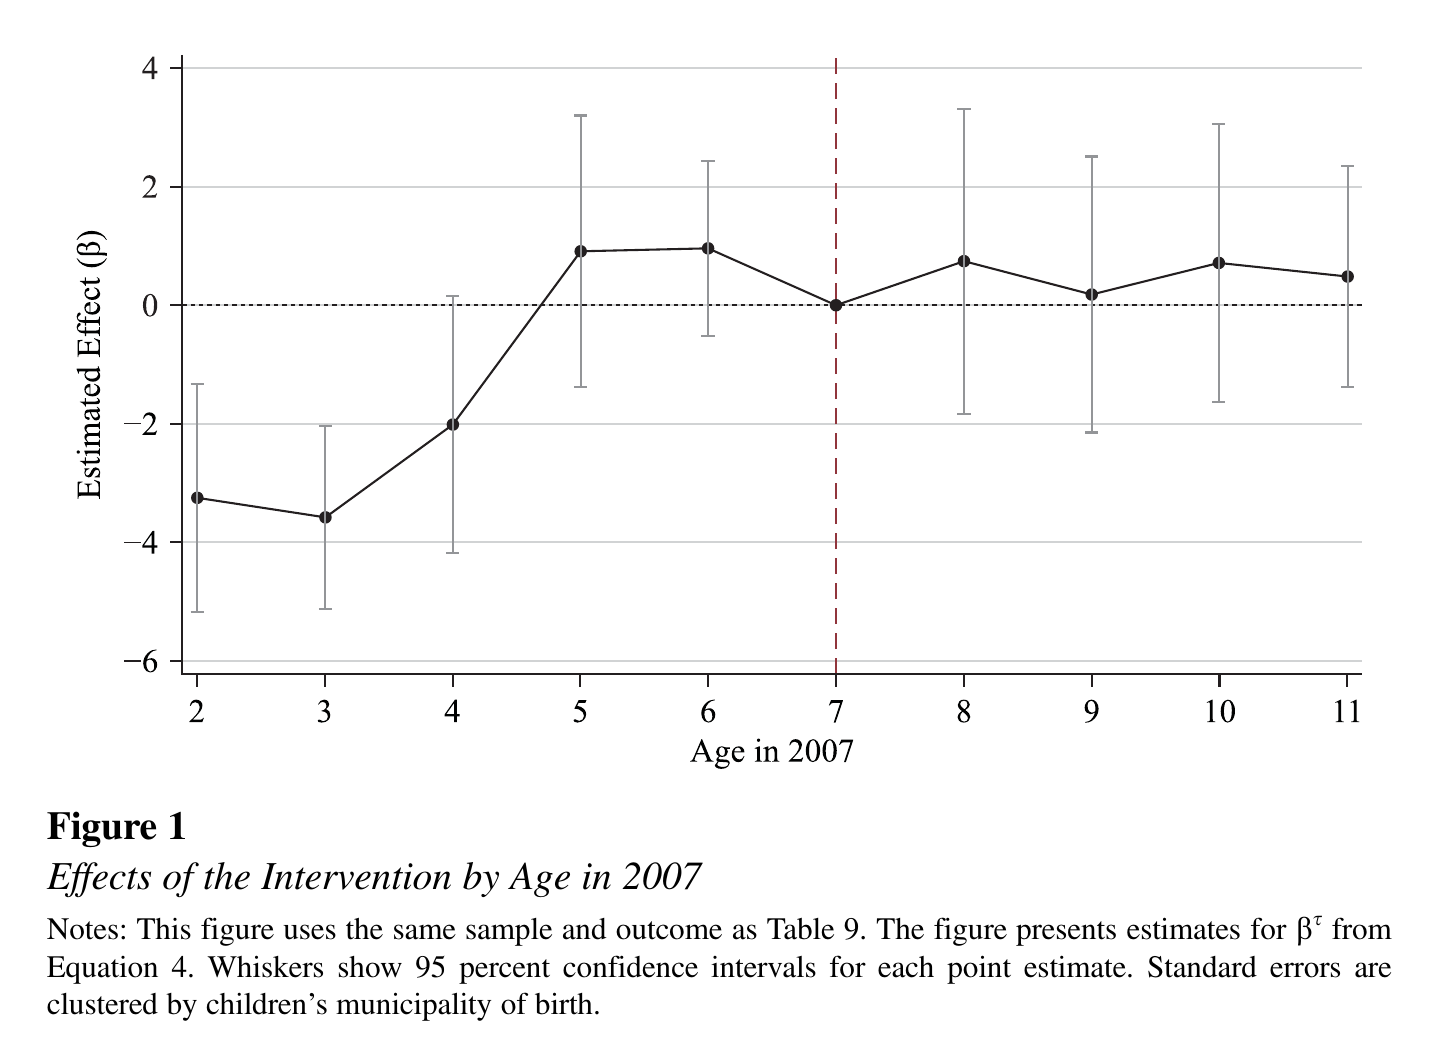
\includegraphics[width=.6\textwidth]{page-38.png}
  \end{figure}
\end{frame}

\begin{frame}{Policy Effects on the Intergenerational Association}
  \begin{itemize}
    \item \textbf{Baseline parent-child association} (control municipalities, ineligible cohort): 9.7 pp
    \begin{itemize}
      \item Very close to 9.8 pp in the full-population analysis
    \end{itemize}
    \item \textbf{Treatment effect ($\hat\beta$):} $-3.8$ pp (statistically significant at 1\%)
    \begin{itemize}
      \item Program \textbf{reduced the parent-child mental health association by 39\%}
    \end{itemize}
    \item Robust to intensive margin transformation (Panel B): $-1.1$ sickness leave days per year
    \item Robust to controlling for municipal trends in health services (Panel C)
    \item Most affected: youngest children at the start of the program (ages 2--4 in 2007)
    \begin{itemize}
      \item Longer exposure and earlier age $\Rightarrow$ larger effects
    \end{itemize}
  \end{itemize}
\end{frame}

\begin{frame}{Effects of the Pilot Program on Intergenerational Persistence}
  \scriptsize
  \begin{tabular}{lccccc}
    \toprule
    & All & College & No College & Males & Females \\
    & (1) & (2) & (3) & (4) & (5) \\
    \midrule
    \multicolumn{6}{l}{\textit{Panel A: Baseline}} \\[2pt]
    $\mathbf{1}$[Parental MH]
      & 9.730$^{***}$ & 8.983$^{***}$ & 10.104$^{***}$ & 8.699$^{***}$ & 10.840$^{***}$ \\
      & (0.461) & (0.532) & (0.671) & (0.669) & (0.905) \\
    $\mathbf{1}$[Parental MH] $\times$ (Age$_{2007}\leq 6$) $\times$ Pilot
      & $-$3.796$^{***}$ & $-$6.210$^{***}$ & $-$2.141 & $-$3.603$^{**}$ & $-$3.916$^{***}$ \\
      & (0.927) & (1.307) & (1.390) & (1.574) & (1.253) \\
    \midrule
    \multicolumn{6}{l}{\textit{Panel B: Duration}} \\[2pt]
    $\mathbf{1}$[Parental MH]
      & 9.801$^{***}$ & 8.965$^{***}$ & 10.148$^{***}$ & 8.649$^{***}$ & 11.036$^{***}$ \\
      & (0.466) & (0.545) & (0.656) & (0.730) & (0.943) \\
    $\mathbf{1}$[Parental MH] $\times$ Duration $\times$ Pilot
      & $-$1.114$^{***}$ & $-$2.425$^{***}$ & $-$0.568 & $-$1.403$^{***}$ & $-$0.795$^{*}$ \\
      & (0.277) & (0.488) & (0.341) & (0.507) & (0.403) \\
    \midrule
    \multicolumn{6}{l}{\textit{Panel C: Municipality trends}} \\[2pt]
    $\mathbf{1}$[Parental MH]
      & 9.703$^{***}$ & 9.007$^{***}$ & 10.076$^{***}$ & 8.673$^{***}$ & 10.804$^{***}$ \\
      & (0.457) & (0.535) & (0.671) & (0.667) & (0.887) \\
    $\mathbf{1}$[Parental MH] $\times$ (Age$_{2007}\leq 6$) $\times$ Pilot
      & $-$3.778$^{***}$ & $-$6.145$^{***}$ & $-$2.137 & $-$3.610$^{**}$ & $-$3.866$^{***}$ \\
      & (0.920) & (1.327) & (1.388) & (1.558) & (1.242) \\
    \midrule
    $N$ & 129,683 & 60,596 & 69,087 & 66,074 & 63,609 \\
    \bottomrule
    \end{tabular}
  \end{frame}

\begin{frame}{Heterogeneity: Who Benefits Most?}
  \begin{itemize}
    \item \textbf{By parental education:}
    \begin{itemize}
      \item College-educated: $-6.2$ pp treatment effect (significant at 1\%)
      \item Non-college: $-2.1$ pp (statistically insignificant)
    \end{itemize}
    \item Pilot was more effective for children of college-educated parents
    \begin{itemize}
      \item Possibly: better ability to navigate and utilize offered services
      \item Policy implication: \textbf{reduces average} parent-child MH association but \textbf{increases within-generation inequality} in mental health outcomes
    \end{itemize}
    \item \textbf{By child gender:} broadly similar effects for boys and girls on extensive margin; 77\% larger for boys on intensive margin
    \begin{itemize}
      \item Boys may be more responsive to positive inputs, especially in childhood (Autor et al.\ 2019)
    \end{itemize}
    \item Authors flag this as a \textbf{cautionary tale} for policymakers: interventions that reduce average persistence can still widen inequality within the affected generation
  \end{itemize}
\end{frame}

% -------------------------------------------------------
\section{Conclusion}
% -------------------------------------------------------

\begin{frame}{Main Takeaways}
  \begin{itemize}
    \item \textbf{Persistence is substantial:} parental MH diagnosis raises child MH probability by 9.3 pp (40\% of control mean); stable across extensive and intensive margins and to extensive robustness checks
    \item \textbf{Dynasty matters:} focusing only on parents understates intergenerational mental health persistence by 42\%; social (not just genetic) transmission is implicated
    \item \textbf{Mental $\approx$ physical:} MH and physical health intergenerational associations are broadly similar --- mental health is not uniquely persistent or uniquely genetic
    \item \textbf{Policy can work:} a low-touch Norwegian pilot reduced the parent-child MH association by 39\%, with largest effects for youngest children
    \item \textbf{But equity matters:} gains accrued primarily to children of college-educated parents; the pilot may have increased inequality within the treated generation
  \end{itemize}
\end{frame}

\begin{frame}{Policy Implications and Future Directions}
  \begin{itemize}
    \item \textbf{Implication 1:} Standard program evaluations that stop at the directly treated generation understate the returns to mental health investments
    \item \textbf{Implication 2:} Light-touch, early-childhood interventions targeting children of MH-diagnosed parents can be cost-effective --- the 2010 national law scaled this approach
    \item \textbf{Implication 3:} Accounting for extended family links is important for understanding the \emph{full} burden of mental illness on society
    \item \textbf{Open questions for future research:}
    \begin{itemize}
      \item Causal mechanisms: exogenous shocks to parental MH (e.g., job loss, health shocks) on child outcomes
      \item Do the gains from the program extend beyond mental health to labor market outcomes?
      \item Optimal design of interventions that reduce average persistence \emph{and} inequality simultaneously
    \end{itemize}
  \end{itemize}
\end{frame}

\end{document}
